%%This is a very basic article template.
%%There is just one section and two subsections.
\documentclass[pdftex,11pt,a4paper]{article}

\usepackage{graphicx}
\usepackage{float}

\begin{document}

\title{Analyzing Model to Model Transformation
	   Tools}
\date{April 23}
\author{Petter Barvik}

\maketitle
\section{Introduction}

Model Driven Engineering(MDE)\cite{France2007} thrives to raise the level of abstraction in
program specification and increase automation in program development. The idea
from MDE is to use models at different levels of abstraction when developing
applications. Therefore raising the level of abstraction in program
specification. This level of abstraction is fulfilled either through extensive
use of models to describe some design patterns in a software application or
through use of standardized models. The first option is probably an element of
MDE that is most common among software engineers. That you implement some aspect
of a system based on a model of a specific language. Unified Modelling Language is
an example of an modelling language often used to describe system design
patterns in an application domain. The second principle of Model Driven
Engineering is to increase automation in program development, and to obtain this
we use something called model transformations. \linebreak 
\newline A model transformation is when we change some source model from one
instance to another instance and end up with a targeted model. We can
distinguish these operations into either endogenous or exogenous model
transformations. In an endogenous model transformation we take one model
expressed in a language and produce a model expressed in the same language.
While in an exogenous model transformation we produce a model expressed in a
different language. It is essential that these models are consistent. This is
obtained through the use of metamodels. A metamodel is an abstraction of a
model, where it defines elements that are used in the model. Models in a
system is consistent if the source and target model conforms to some unique 
metamodel. This way system developers can safely presume that a model has
changed accordingly to its metamodel and therefore is consistent. A target model
can produce two different kind of output models. The first one is code
generation, often referred to Model to Text(M2T) transformation, and it takes
one model and produces implementation code. This is convenient if for example a software
engineer wants to produce source code from a given model. The latter is often
referred to Model to Model(M2M) transformations, that is also the subject of
my master thesis. M2M transformations take a model as input and produces a model
as output. In this article we try and go into depth for some model
transformation tools. These tools are Henshin, AGG and ATL. Henshin and AGG is
build around graph transformation. 

\subsection{The Model Instances}
The task was to take a certain instance of model transformation, in this case
transforming a activity diagram, written in the language UML and
transform it to petri net. We initialize the metamodels to make sure that the
models remain consistent.

\begin{figure}[H]
	\centering
	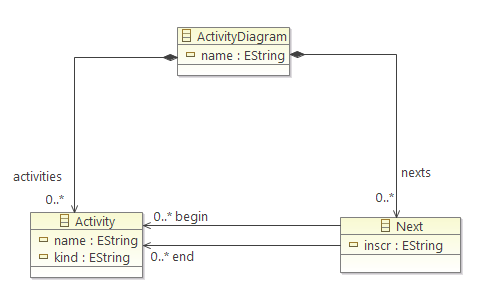
\includegraphics[scale=0.5]{figures/ActivityMetamodel.png}
	\caption{Metamodel of Activity Diagram }
\end{figure}

The metamodel of an activity diagram has an arbitrary number of activity and
next elements. An activity element can have a name and can be of some type kind.
Example of activity types can be decision or simple. The next element can have
an inscription and has the property to either start or end an activity. The
collection of activity and next elements have to have an activity diagram that
they belong to. Now we have defined the metamodel that the source model should
conform to. To keep consistency between the models we need to have a
metamodel for the target model.

\begin{figure}[H]
	\centering
	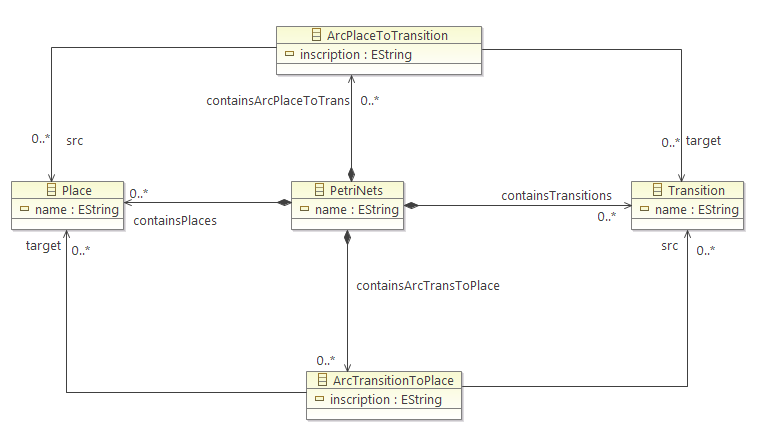
\includegraphics[scale=0.5]{figures/PetriNetsMetamodel.png}
	\caption{Metamodel of Petri nets}
\end{figure}

The metamodel for a petri net consist of places and transitions. A petri net
instance must have a place connected to a transition or the other way around.
But a petri net can never have two of the same types connected with each other.
There also is two nodes that distinguish if the arrow has a place or a
transition as source node and the opposite as target node.

\subsection{Defining a set of rules}
For a transformation language to be able to execute for graph transformations a
set of rules needs to be defined. Through these rules, a transformation
interpreter can act accordingly. 

\subsection{Graph Transformation}
Model transformations can occur through the use of graph transformations, also
referred to graph rewriting.

\section{Henshin}

Henshin provides a model transformation language for the Eclipse Modelling
Framework \cite{Steinberg2009}. With support for both direct 
transformation of EMF single model instances, and translation from source
model to targeted model. The Henshin project is a transformation language with a
provided graphical syntax. With the help of this graphical editor, it provides
the user with an intuitive way of representing rules. The tool also has support 
both endogenous and exogenous transformations.

\subsection{Defining transformation rules}

In Henshin, objects are referred to as nodes and links between objects as edges.
A collection of these nodes and edges form a graph. For each graph, a rule has
to be defined. These rules can have parameters for checking and model
verification. Each rule can be represented as a graph in the graphical
editor. \linebreak
\newline When creating these rules, there has to be a way of distinguishing
elements between the LHS and the RHS. This is done through the use of
a set of predefined tag words, or stereotypes. For handling transformations
either in the pattern graph or the replacement graph, we can use the three
predefined words preserve, create or delete. Forbid and require are used for
defining Negative Application Conditions (NACs) and Positive Application
Conditions (PACs). These actions are supported for nodes, edges and attributes.

\pagebreak
\bibliographystyle{plain} 
\bibliography{Master}

\end{document}
